\section{Benchmark}\label{sec:benchmark}

In this section, we study a wide array of benchmarks.

\subsection{Proximal Gradient Descent vs. Newton}\label{ssec:benchmark:pgd-newton}

In this section, we compare the algorithms presented 
in~\Cref{ssec:pgd,ssec:newton,ssec:newton-abs}
that solve the block update~(\ref{eq:bcd:block-update}).
Recall the objective to solve is
\begin{align*}
    \minimize_{\beta \in \R^p}
    \frac{1}{2} \beta^\top D \beta
    - v^\top \beta
    + \lambda \norm{\beta}_2
\end{align*}
where $D$ is a diagonal matrix with non-negative entries,
$v$ any vector, and $\lambda > 0$.

\Cref{fig:bench:pgd-newton} shows a set of comparisons
of ISTA, FISTA, FISTA with adaptive restart (FISTA-ADA),
Newton, Newton-Brent, and Newton-ABS.
Newton-Brent works exactly the same as Newton-ABS except
the adaptive bisection is replaced with Brent's method.
For all scenarios, the diagonal of $D$ was generated uniformly from $[0.8, 2]$.
In \Cref{fig:bench:pgd-newton:almost_psd}, 1\% of the entries were
regenerated uniformly from $[\num{1e-14}, \num{1e-8}]$.
In \Cref{fig:bench:pgd-newton:very_psd}, 20\% of the entries were
set exactly to zero and 10\% were regenerated from $[\num{1e-14}, \num{1e-8}]$.
The vector $v$ was generated from $\Normal\pr{0, D}$.
Finally, \Cref{fig:bench:pgd-newton:pd,fig:bench:pgd-newton:almost_psd,fig:bench:pgd-newton:very_psd}
used $\lambda=\num{1e-1}$ 
while \Cref{fig:bench:pgd-newton:low_regul} used $\lambda=\num{1e-4}$
with positive definite $D$.
Each setting measures total time, relative time to Newton-ABS,
number of iterations until convergence, and accuracy.
All methods converged before max iterations was reached.
The accuracy comparisons show that all methods properly converged,
with Newton-ABS generally having smaller errors.
The timings had large variance for small number of features,
since most of the time was spent in the scripting language to dispatch the function calls.
Overall, the Newton methods clearly outshine the PGD methods in terms of speed.
The PGD methods generally use around 100 or even 1000 iterations,
however Newton method is consistently using 20 to 30 iterations,
Newton-Brent using 6 to 10 iterations,
and Newton-ABS using 3 to 4 iterations.
The relative speed difference shows that Newton-ABS is anywhere from 3 to 100 times faster
than the PGD methods, 1.5 to 5 times faster than Newton, and around 2 times faster than Newton-Brent,
where the differences become stark as $p$ increases or regularization level decreases.
We also note that the PGD methods and Newton are quite comparable in speed
when the regularization is low. 
Since the blockwise coordinate descent takes a longer time to converge with low regularization
and more groups will be active, the block update must especially be fast in this setting.
Hence, we expect significant improvement to the overall optimizer with Newton-ABS,
as its block update performance seems unaffected.

\begin{figure}
    \centering
    \begin{subfigure}[b]{0.49\textwidth}
        \centering
        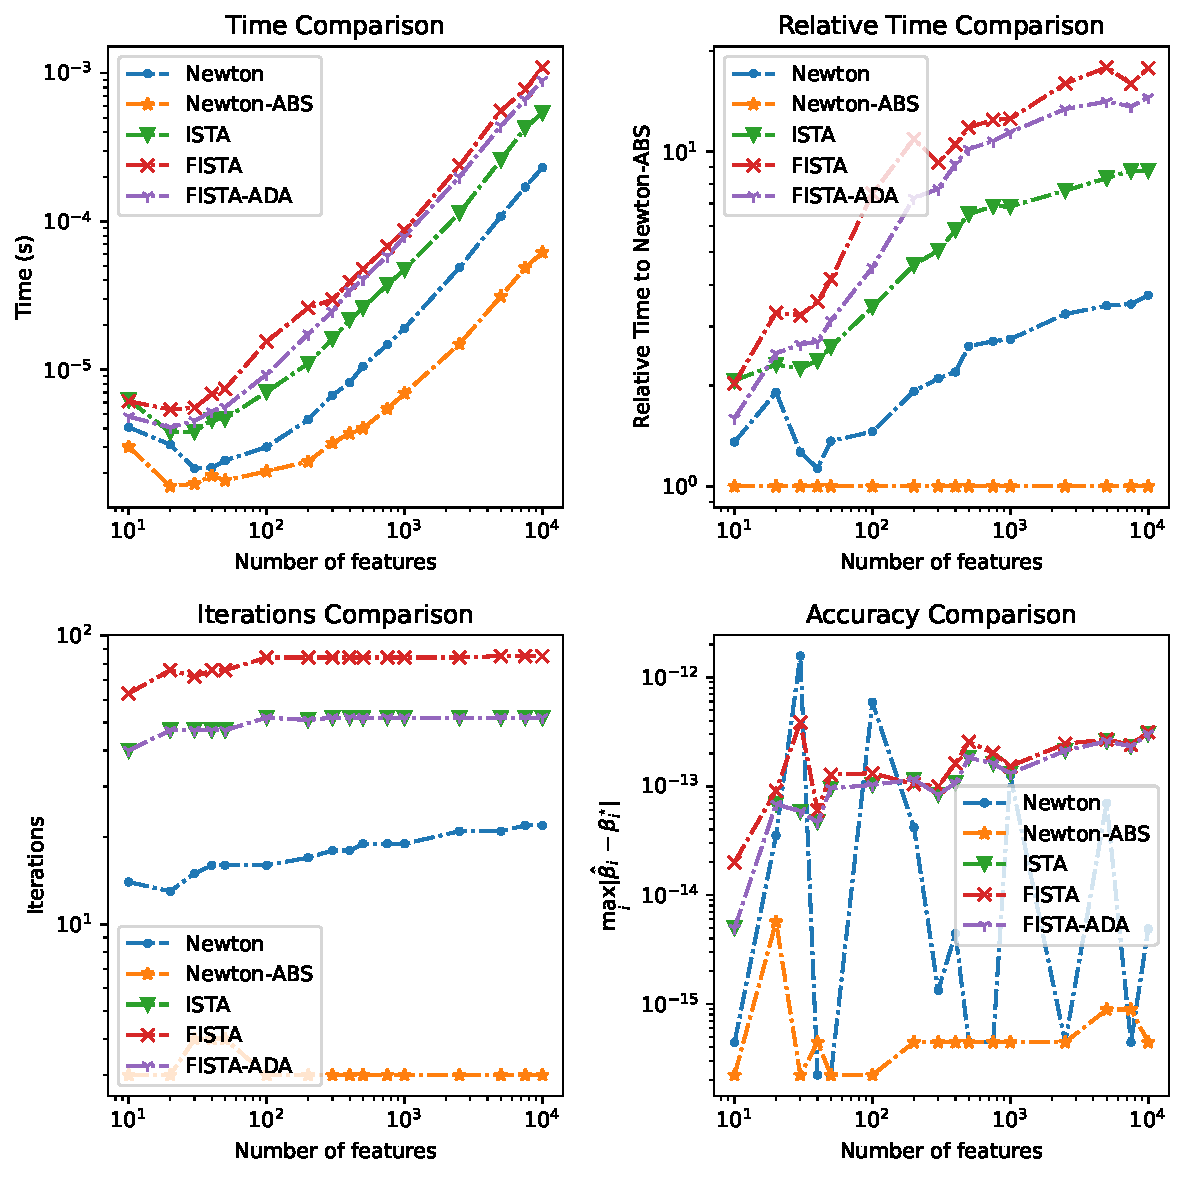
\includegraphics[width=\textwidth]{figures/pgd_newton_pd.pdf}
        \caption{Positive definite}
        \label{fig:bench:pgd-newton:pd}
    \end{subfigure} 
    \hfill
    \begin{subfigure}[b]{0.49\textwidth}
        \centering
        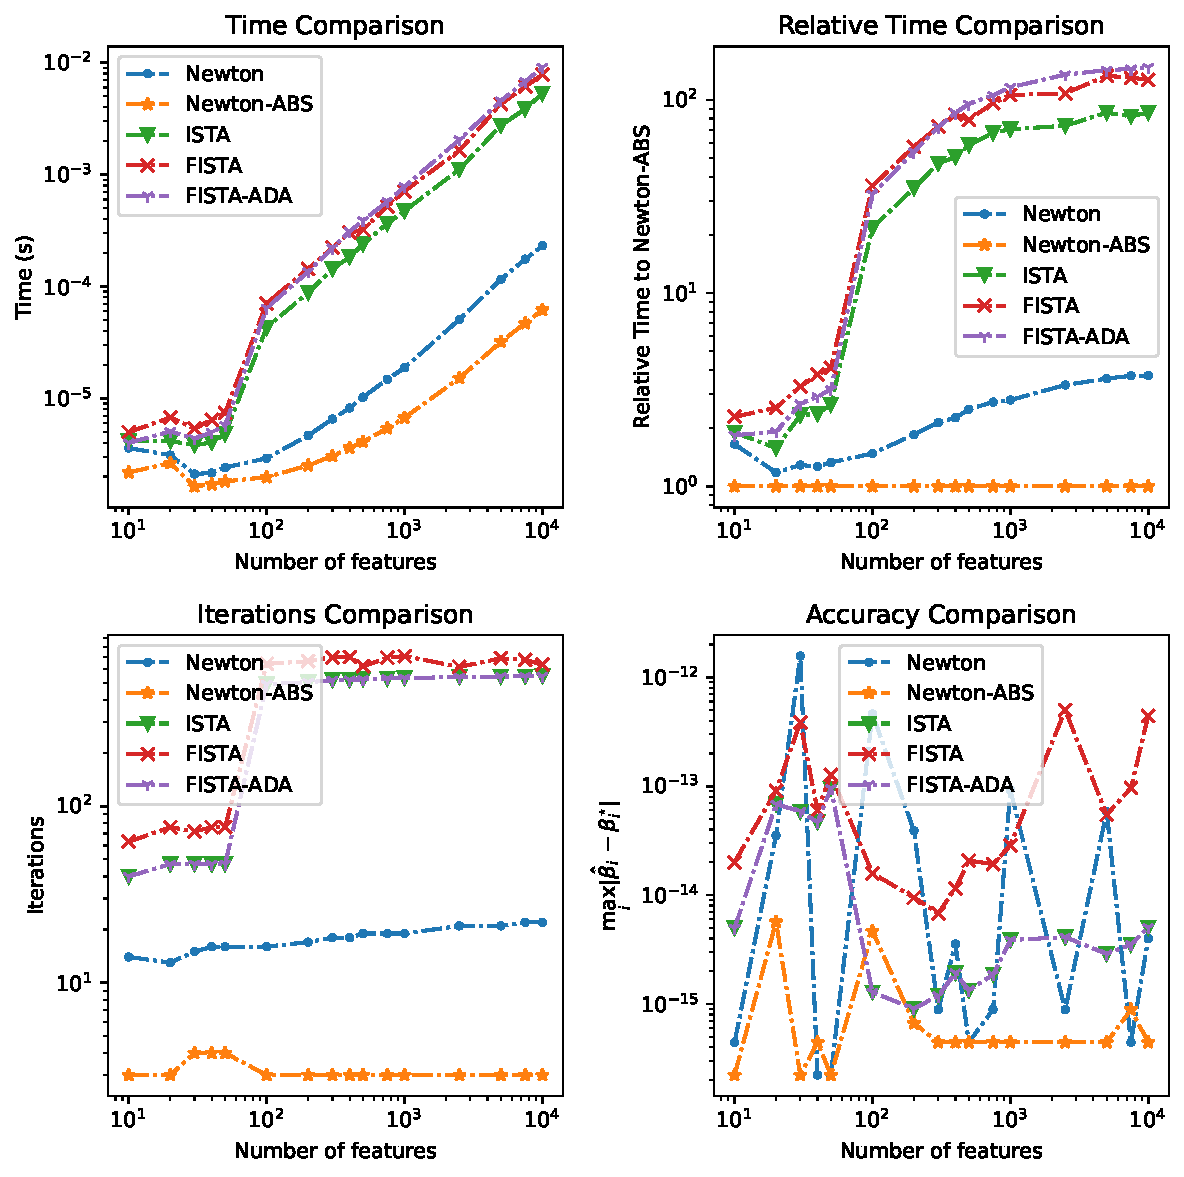
\includegraphics[width=\textwidth]{figures/pgd_newton_almost_psd.pdf}
        \caption{Almost semi-definite}
        \label{fig:bench:pgd-newton:almost_psd}
    \end{subfigure} 
    \\
    \begin{subfigure}[b]{0.49\textwidth}
        \centering
        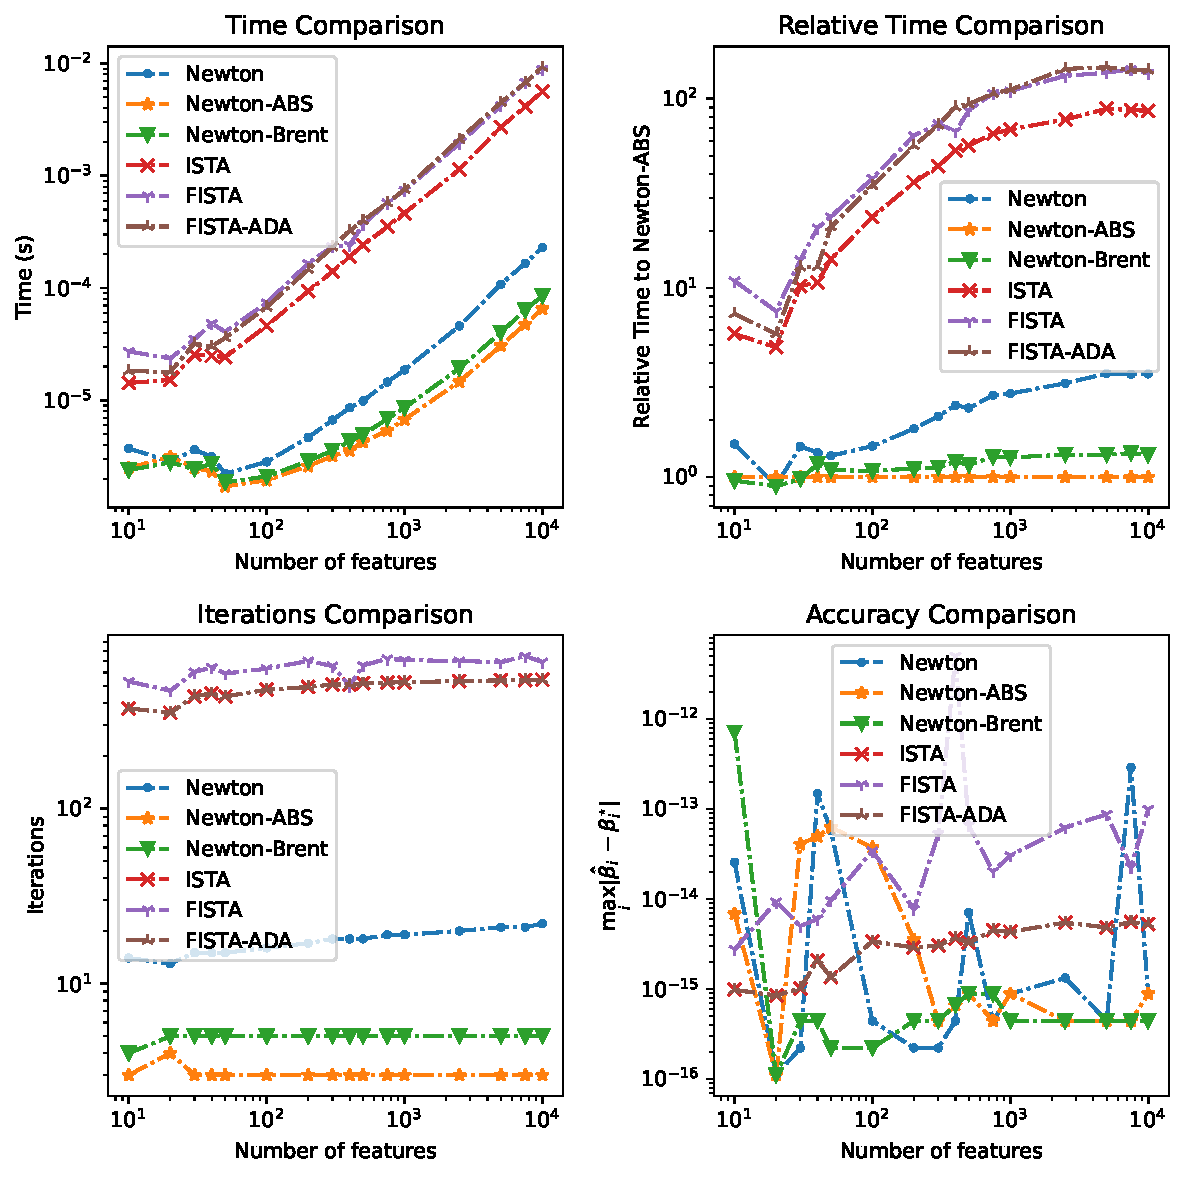
\includegraphics[width=\textwidth]{figures/pgd_newton_very_psd.pdf}
        \caption{Very semi-definite}
        \label{fig:bench:pgd-newton:very_psd}
    \end{subfigure} 
    \hfill
    \begin{subfigure}[b]{0.49\textwidth}
        \centering
        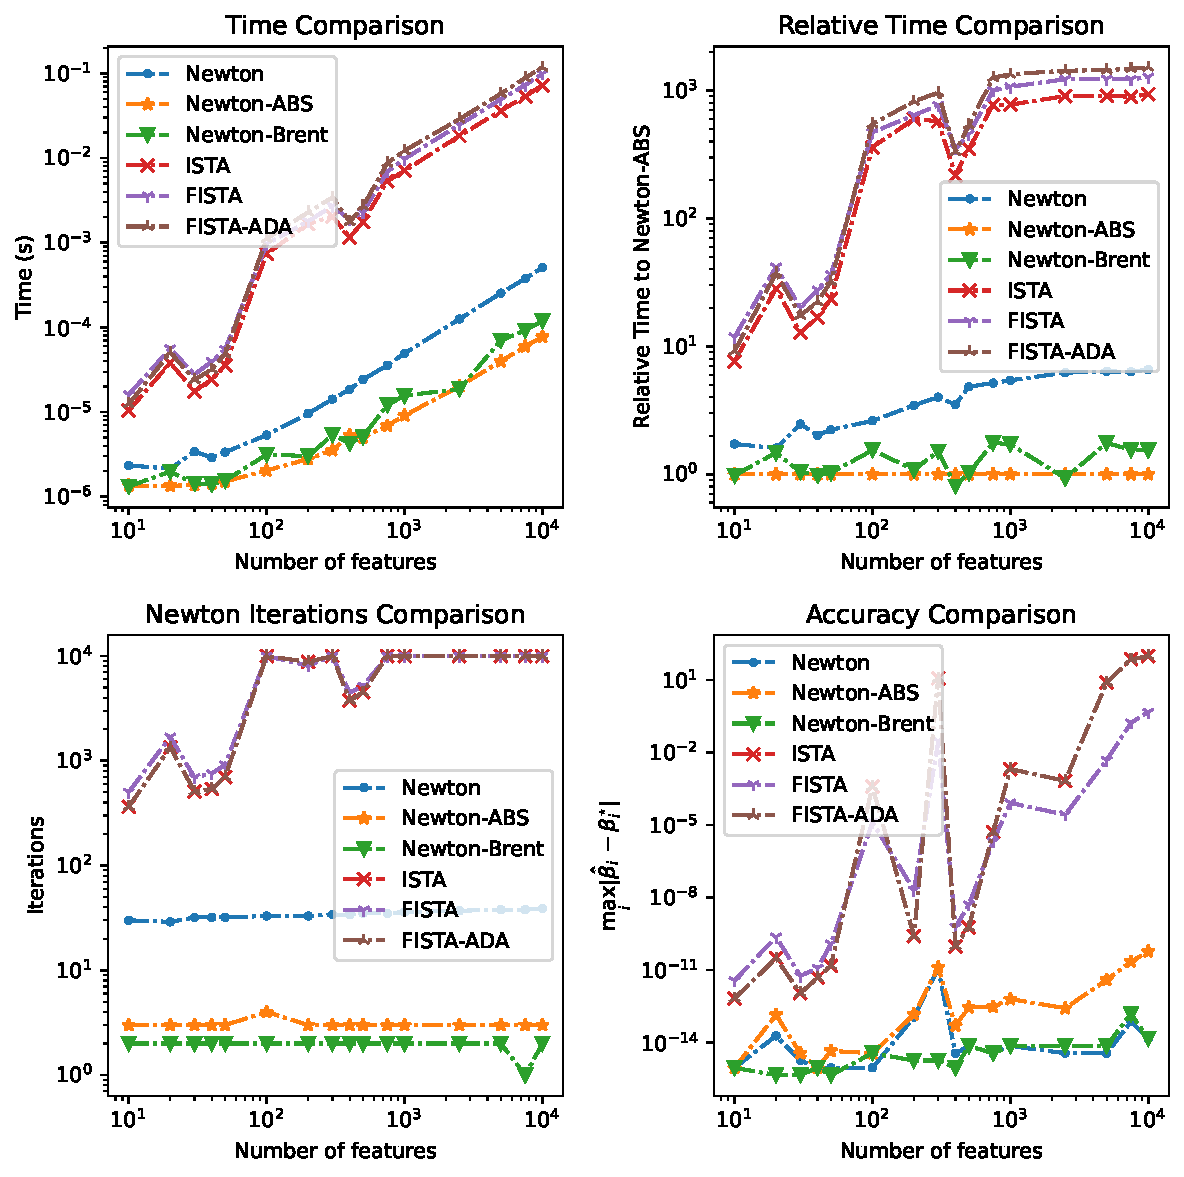
\includegraphics[width=\textwidth]{figures/pgd_newton_low_regul.pdf}
        \caption{Positive definite and low regularization}
        \label{fig:bench:pgd-newton:low_regul}
    \end{subfigure} 
    \caption{%
        \Cref{%
            fig:bench:pgd-newton:low_regul,%
            fig:bench:pgd-newton:almost_psd,%
            fig:bench:pgd-newton:pd,%
            fig:bench:pgd-newton:very_psd%
        }
        show a comparison of time, relative time, number of iterations, and accuracy
        across different algorithms.
        \Cref{%
            fig:bench:pgd-newton:almost_psd,%
            fig:bench:pgd-newton:pd,%
            fig:bench:pgd-newton:very_psd%
        } fixed $\lambda=\num{1e-1}$ while 
        \Cref{fig:bench:pgd-newton:pd} fixed $\lambda=\num{1e-4}$.
        The difference across
        \Cref{%
            fig:bench:pgd-newton:almost_psd,%
            fig:bench:pgd-newton:pd,%
            fig:bench:pgd-newton:very_psd%
        } is the degree of singularity of $D$.
        \Cref{fig:bench:pgd-newton:pd} used a positive definite $D$,
        \Cref{fig:bench:pgd-newton:almost_psd} used a positive definite $D$ with
        some eigenvalues close to $0$ (but not exactly), and
        \Cref{fig:bench:pgd-newton:very_psd} used a positive semi-definite $D$
        with some eigenvalues exactly at $0$, some close to $0$, and some sufficiently positive.
        The accuracy comparisons show that all methods properly converged,
        with Newton-ABS generally having smaller errors.
        Overall, the Newton methods clearly outshine the PGD methods in terms of speed
        with Newton-ABS in the obvious lead.
    }
    \label{fig:bench:pgd-newton}
\end{figure}
